\documentclass[11pt]{article}
\usepackage{graphicx}
\usepackage{float}
\usepackage{hyperref}
\usepackage{natbib}
\usepackage{listings}
\usepackage{xcolor}
\usepackage[dvipsnames]{xcolor}
\usepackage[svgnames]{xcolor}
\usepackage{amsmath} % For the equation* environment
\usepackage{amssymb}
\usepackage{caption}
\usepackage{subcaption}

\hypersetup{
    colorlinks=true,
    linkcolor=red,
    filecolor=cyan,      
    urlcolor=orange,
    pdftitle={Overleaf Example},
    pdfpagemode=FullScreen,
    }

\setlength{\textwidth}{6.5in}
\setlength{\headheight}{0in}
\setlength{\textheight}{8.0in}
\setlength{\hoffset}{0in}
\setlength{\voffset}{0in}
\setlength{\oddsidemargin}{0in}
\setlength{\evensidemargin}{0in}

\lstdefinestyle{txtstyle}{
    basicstyle=\ttfamily\small,
    breaklines=true,
    backgroundcolor=\color{Bisque}
}
\lstset{style = txtstyle}

\definecolor{codegreen}{rgb}{0,0.6,0}
\definecolor{codegray}{rgb}{0.5,0.5,0.5}
\definecolor{codepurple}{rgb}{0.58,0,0.82}
\definecolor{backcolour}{rgb}{0.95,0.95,0.92}

\lstdefinestyle{mystyle}{
    backgroundcolor=\color{backcolour},   
    commentstyle=\color{codegreen},
    keywordstyle=\color{magenta},
    numberstyle=\tiny\color{codegray},
    stringstyle=\color{codepurple},
    basicstyle=\ttfamily\footnotesize,
    breakatwhitespace=false,         
    breaklines=true,                 
    captionpos=b,                    
    keepspaces=true,                                   
    numbersep=5pt,                  
    showspaces=false,                
    showstringspaces=false,
    showtabs=false,                  
    tabsize=2
}

\title{Computational Physics ps-10 Report}
  
\author{Tongzhou Wang, \\ GitHub account: TZW56203, repository: phys-ga2000. \\ \url{https://github.com/TZW56203/phys-ga2000}}

\date{December 10, 2024}

\begin{document}

\maketitle

\section{Problem 1}

\subsection{Part (a)}
Figure \ref{fig:CN} shows the wave function at various times computed using the Crank-Nicolson method.
\begin{figure}[H]
    \centering
    \begin{subfigure}[H]{0.48\textwidth}
        \centering
        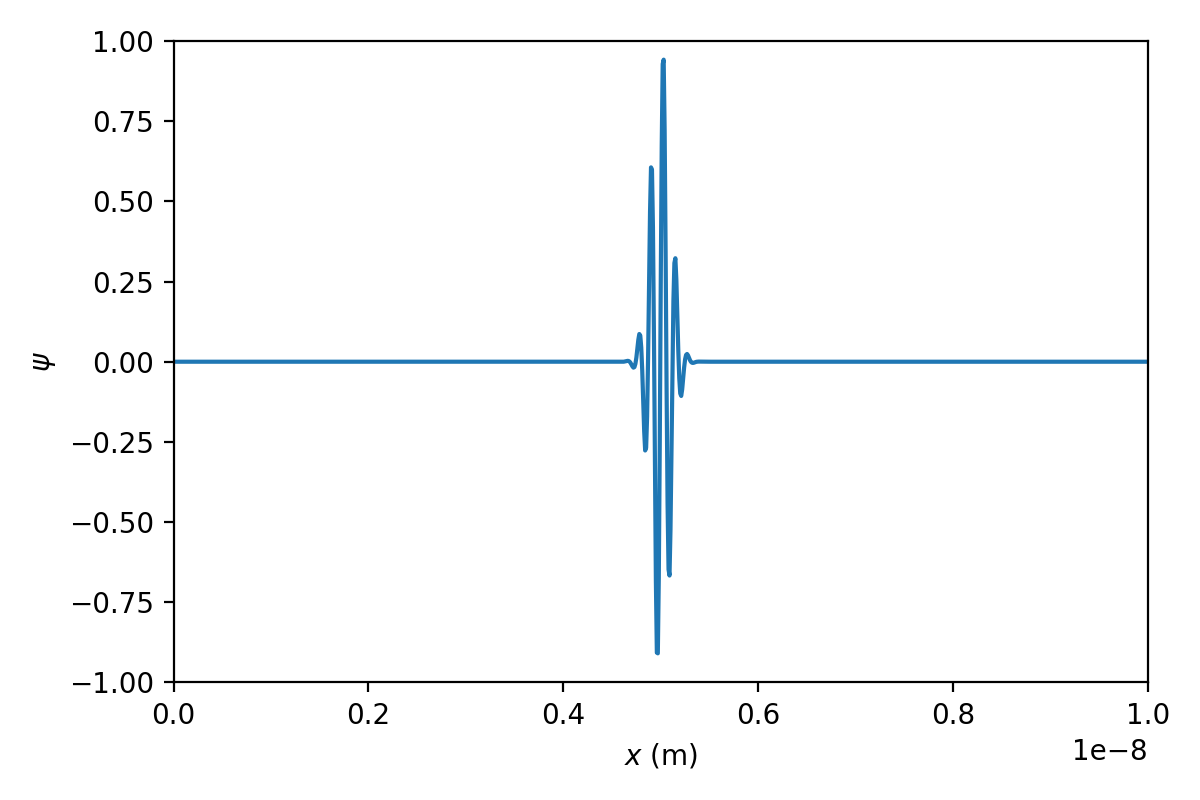
\includegraphics[width=\textwidth]{Figs/ps-10-1-0.png}
    \end{subfigure}
    \hfill
    \centering
    \begin{subfigure}[H]{0.48\textwidth}
        \centering
        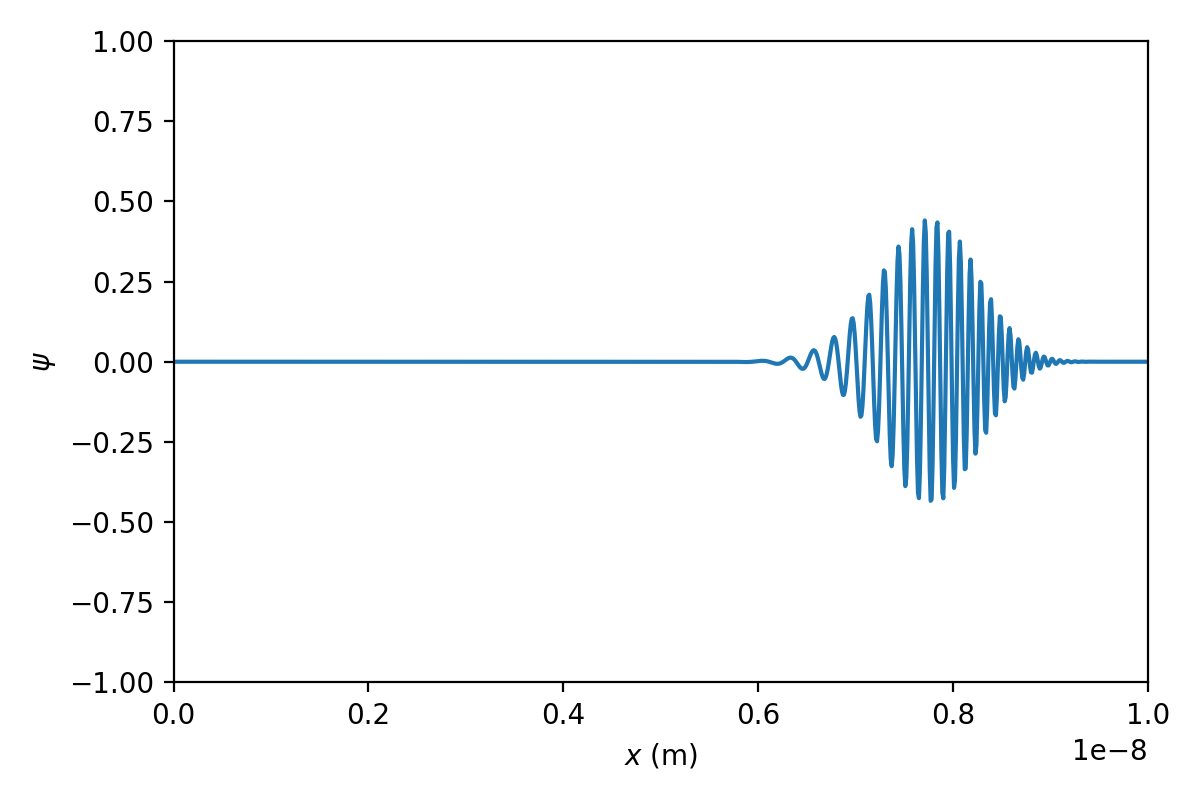
\includegraphics[width=\textwidth]{Figs/ps-10-1-1.png}
    \end{subfigure}

    \begin{subfigure}[H]{0.48\textwidth}
        \centering
        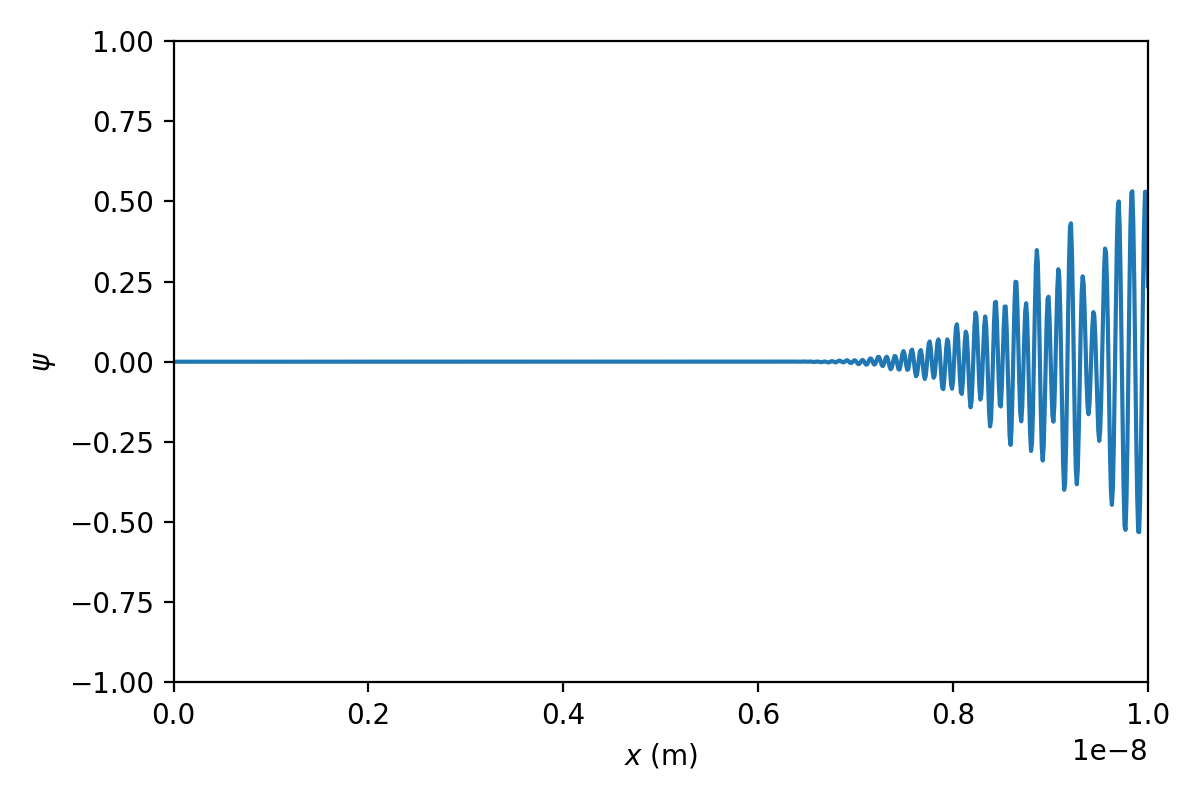
\includegraphics[width=\textwidth]{Figs/ps-10-1-2.png}
    \end{subfigure}
    \hfill
    \begin{subfigure}[H]{0.48\textwidth}
        \centering
        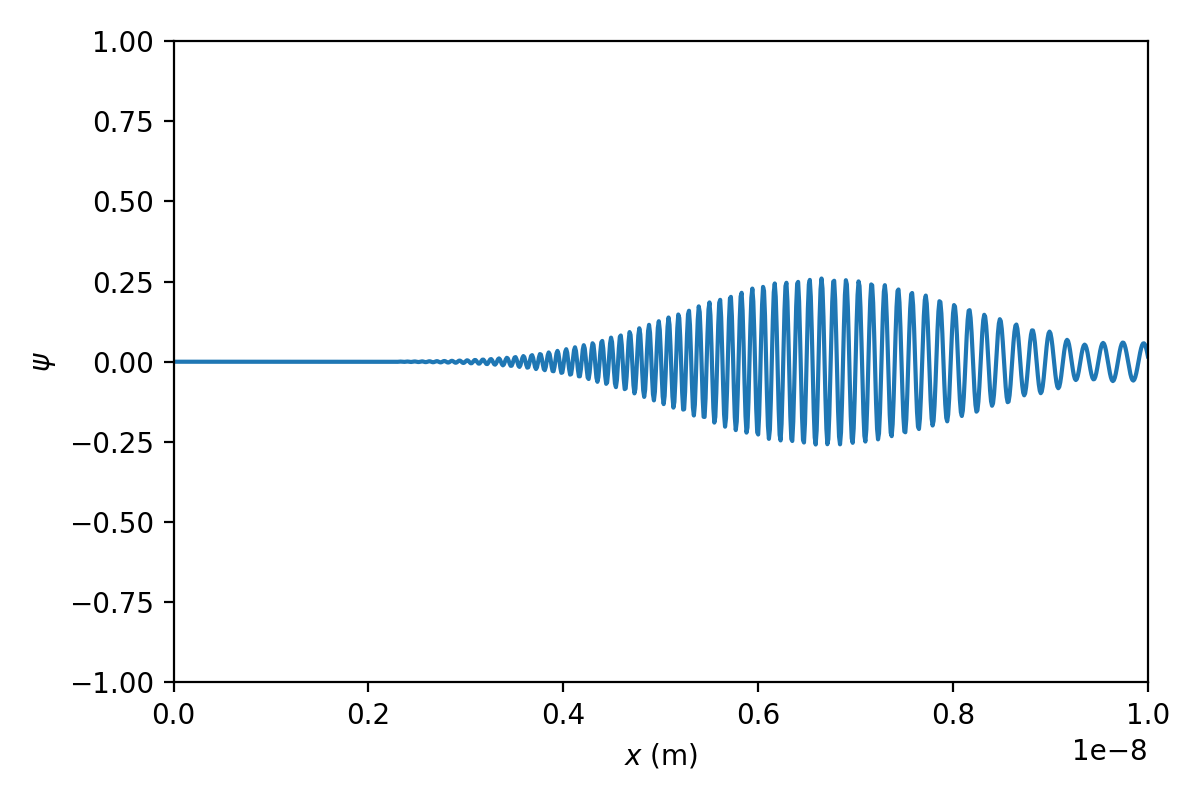
\includegraphics[width=\textwidth]{Figs/ps-10-1-3.png}
    \end{subfigure}
    \caption{Wave function at various times computed using the Crank-Nicolson method.}
    \label{fig:CN}
\end{figure}

\subsection{Part (b)}
Please see the \texttt{ps-10-1.gif} file in my GitHub repository for the animation.

\subsection{Part (c)}\label{explain}
We can observe from Figure \ref{fig:CN} and the animation that the wave function of the particle spreads out, moves to the edge of the box, and is reflected back. This indicates that the particle is reflected back by the infinite square well as expected.

\section{Problem 2}

\subsection{Part (a) and (b)}
Figure \ref{fig:test} shows the wave function at $t = 10^{-16}$ s computed using the spectral method.
\begin{figure}[H]
    \centering
    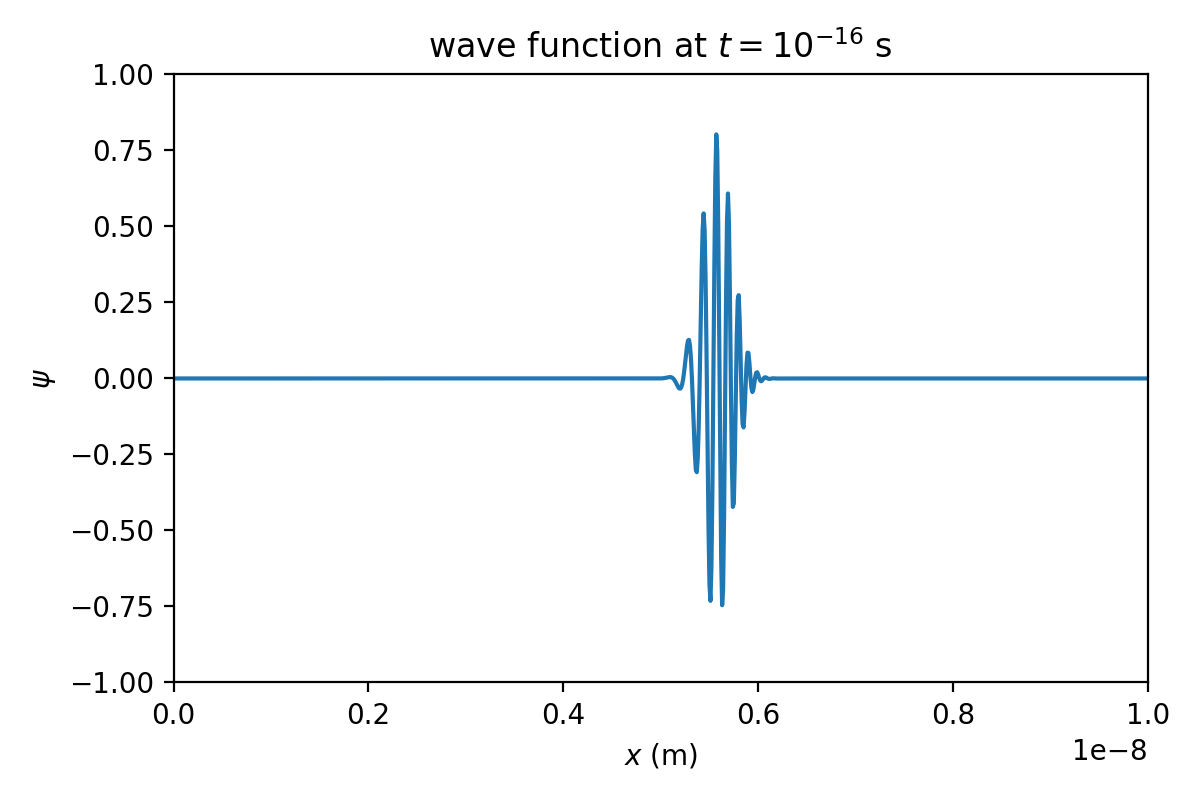
\includegraphics[scale = 0.7]{Figs/ps-10-2-test.png}
    \caption{Wave function at $t = 10^{-16}$ s computed using the spectral method.}
    \label{fig:test}
\end{figure}

Figure \ref{fig:spectral} shows the wave function at various times computed using the spectral method. The behavior of the wave function is similar to that computed using the Crank-Nicolson method in Figure \ref{fig:CN}.
\begin{figure}[H]
    \centering
    \begin{subfigure}[H]{0.48\textwidth}
        \centering
        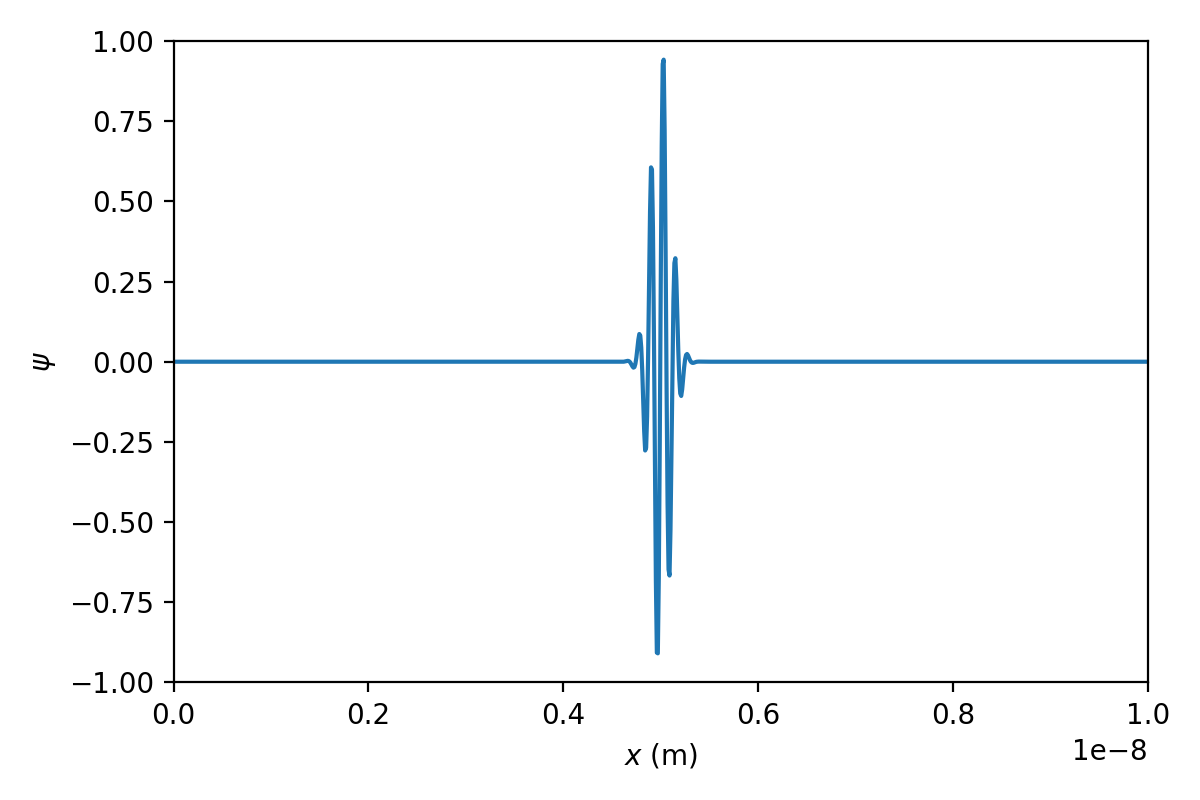
\includegraphics[width=\textwidth]{Figs/ps-10-2-0.png}
    \end{subfigure}
    \hfill
    \centering
    \begin{subfigure}[H]{0.48\textwidth}
        \centering
        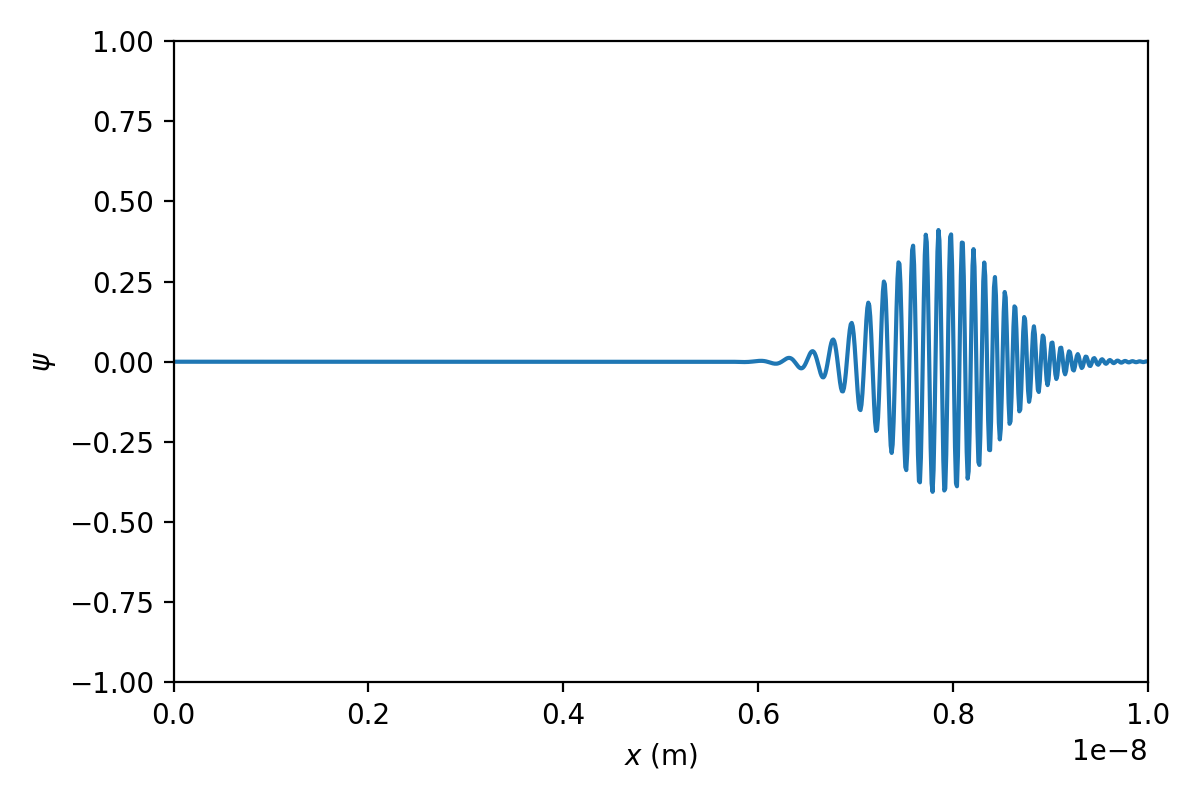
\includegraphics[width=\textwidth]{Figs/ps-10-2-1.png}
    \end{subfigure}

    \begin{subfigure}[H]{0.48\textwidth}
        \centering
        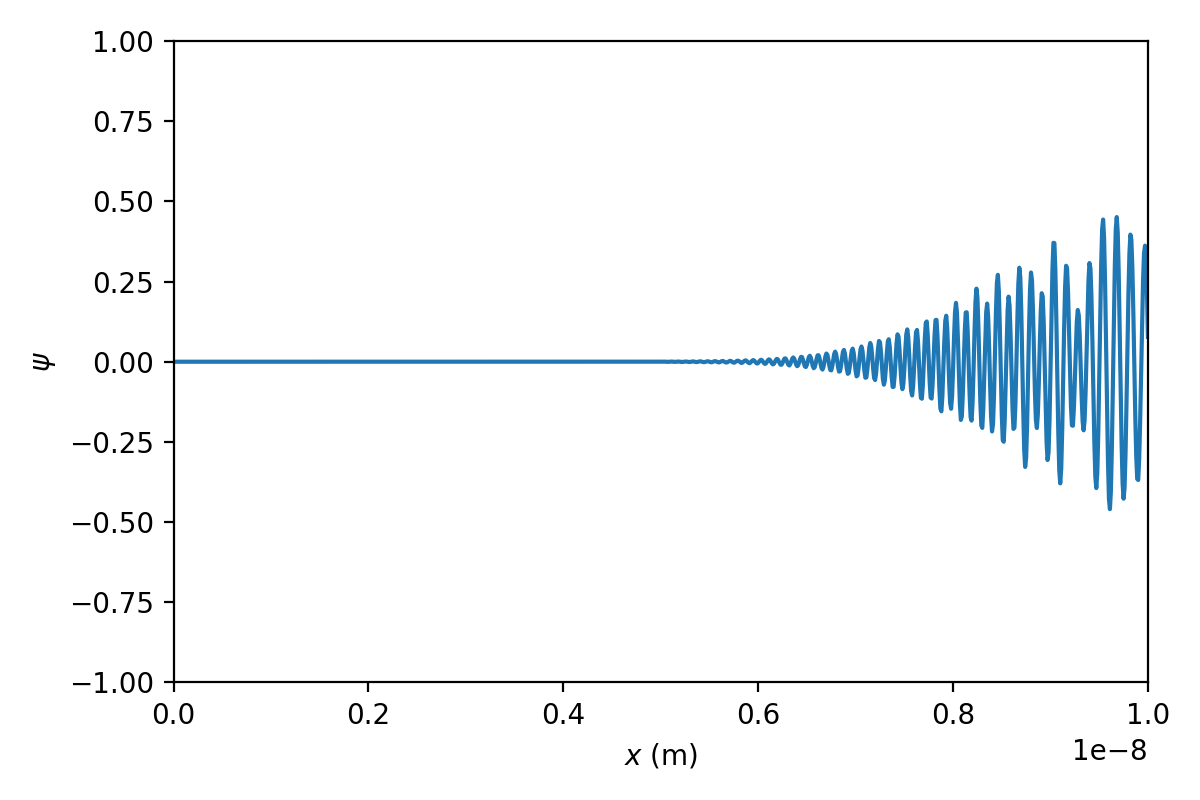
\includegraphics[width=\textwidth]{Figs/ps-10-2-2.png}
    \end{subfigure}
    \hfill
    \begin{subfigure}[H]{0.48\textwidth}
        \centering
        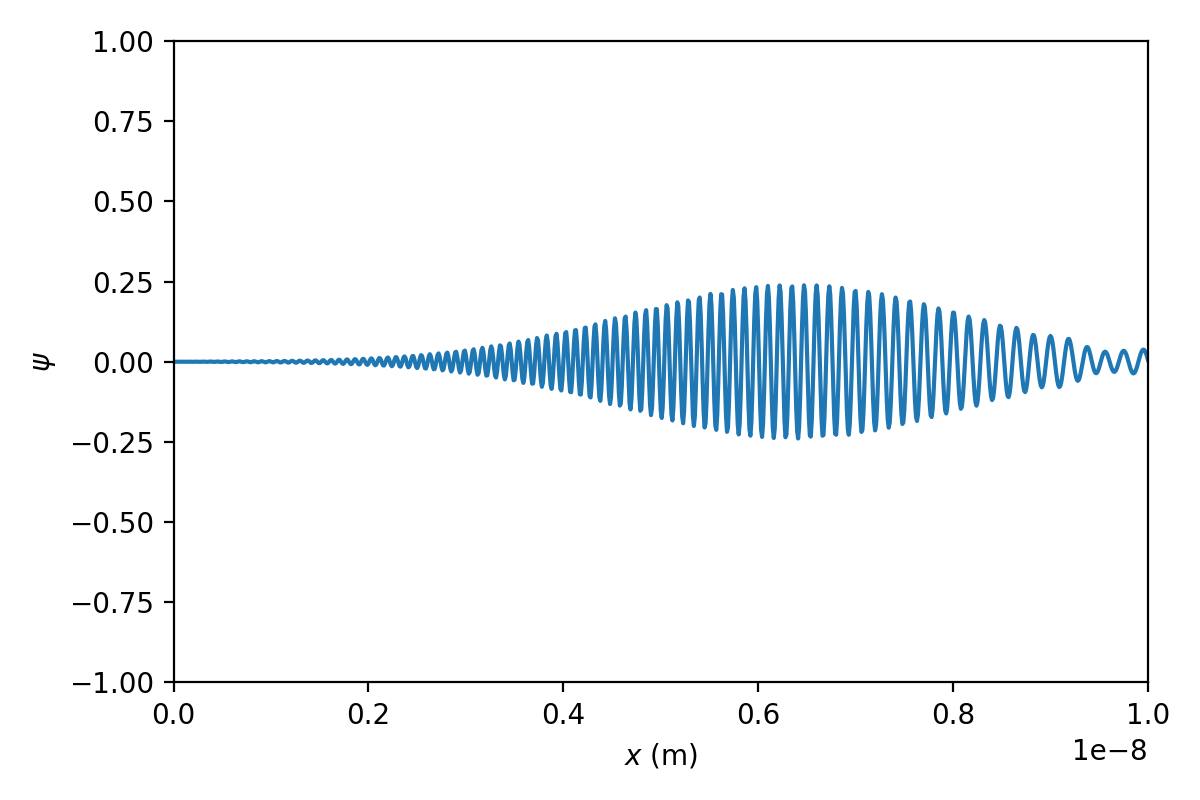
\includegraphics[width=\textwidth]{Figs/ps-10-2-3.png}
    \end{subfigure}
    \caption{Wave function at various times computed using the spectral method.}
    \label{fig:spectral}
\end{figure}

\subsection{Part (c)}
Please see the \texttt{ps-10-2.gif} file in my GitHub repository for the animation.

\subsection{Part (d)}
Identical to Subsection \ref{explain}.

\end{document}
